\documentclass[10pt, aspectratio=169]{beamer}

\usetheme{Madrid}
\usecolortheme{default}

\usepackage{amsmath, amssymb, amsthm}
\usepackage{tikz}
\usetikzlibrary{math}
\usetikzlibrary{shapes.misc}
\usepackage{pgfplots}
\usetikzlibrary{calc}
\usetikzlibrary{arrows.meta,backgrounds,fit,positioning}
\usepgfplotslibrary{patchplots}
\usepgfplotslibrary{fillbetween}
\pgfplotsset{%
    layers/standard/.define layer set={%
        background,axis background,axis grid,axis ticks,axis lines,axis tick labels,pre main,main,axis descriptions,axis foreground%
    }{
        grid style={/pgfplots/on layer=axis grid},%
        tick style={/pgfplots/on layer=axis ticks},%
        axis line style={/pgfplots/on layer=axis lines},%
        label style={/pgfplots/on layer=axis descriptions},%
        legend style={/pgfplots/on layer=axis descriptions},%
        title style={/pgfplots/on layer=axis descriptions},%
        colorbar style={/pgfplots/on layer=axis descriptions},%
        ticklabel style={/pgfplots/on layer=axis tick labels},%
        axis background@ style={/pgfplots/on layer=axis background},%
        3d box foreground style={/pgfplots/on layer=axis foreground},%
    },
}
\pgfplotsset{compat=1.18}
\usepackage{graphicx}
\usepackage{mathtools}
\usepackage{bbm}

\title[Non-Singularity of the GD Map]{Non-Singularity of the Gradient Descent Map for Neural Networks with Piecewise Analytic Activations}
\author[A. Crăciun \& D. Ghoshdastidar]{Alexandru Crăciun \and Debarghya Ghoshdastidar \\ \vspace{0.3cm} \small \textit{Presented by Ian Chi, slides made with assistance by Gemini 2.1}}
\institute[NeurIPS 2025]{39th Conference on Neural Information Processing Systems (NeurIPS 2025)}
\date{\today}

% Definitions and Theorems
\theoremstyle{definition}
\newtheorem{defn}{Definition}
\newtheorem{thm}{Theorem}
\newtheorem{lem}{Lemma}
\newtheorem{cor}{Corollary}
\newtheorem{prop}{Proposition}
\newtheorem{asm}{Assumption}

\begin{document}
% \useouthertheme{smoothbars}

\begin{frame}
    \titlepage
\end{frame}

\begin{frame}{Outline}
    \tableofcontents[hideallsubsections]
\end{frame}

\section{Introduction \& Optimization Dynamics}

\begin{frame}{The Central Problem: Training Deep Networks}
    \begin{itemize}
        \item Let $f_\theta: \mathbb{R}^d \to \mathbb{R}^k$ be a neural network parameterized by weights and biases $\theta \in \mathbb{R}^p$.
        \item For a dataset $\{(x_i, y_i)\}_{i=1}^N$ and a loss function $\ell$, the empirical risk is:
        \begin{equation*}
            L(\theta) = \frac{1}{N} \sum_{i=1}^N \ell(f_\theta(x_i), y_i)
        \end{equation*}
        \item The Gradient Descent (GD) update rule is defined as a discrete-time dynamical system:
        \begin{equation*}
            \theta_{t+1} = G_\eta(\theta_t) \coloneqq \theta_t - \eta \nabla L(\theta_t)
        \end{equation*}
        where $\eta > 0$ is the step-size (learning rate) and $G_\eta: \mathbb{R}^p \to \mathbb{R}^p$ is the \textbf{GD map}.
    \end{itemize}
\end{frame}

\begin{frame}{Saddle Points in High Dimensions}
    \begin{itemize}
        \item The loss landscape of overparameterized neural networks is highly non-convex.
        \item Critical points ($\nabla L(\theta) = 0$) can be local minima, local maxima, or saddle points.
        \item In high-dimensional spaces ($p \gg 1$), saddle points are exponentially more prevalent than local minima (Dauphin et al., 2014).
        % \item \textbf{Strict Saddle Property:} A saddle point $\theta^*$ is strict if the Hessian $\nabla^2 L(\theta^*)$ has at least one strictly negative eigenvalue ($\lambda_{\min} < 0$).
        \item \textbf{Key Question:} Why doesn't GD get trapped in these ubiquitous saddle points?
        % \item Papers proving results assume non-singularity.
    \end{itemize}
\end{frame}

% \begin{frame}{Avoiding Saddle Points (Lee et al., 2016)}
%     \begin{itemize}
%         \item A landmark result by Lee et al. showed that GD randomly initialized will almost surely converge to local minimizers, avoiding strict saddle points.
%         \item \textbf{Core Mathematical Machinery:} The Stable Manifold Theorem.
%         \item For a strict saddle point $\theta^*$, the set of initializations that converge to $\theta^*$ is confined to a \textit{stable manifold} $W^s(\theta^*)$.
%         \item If $W^s(\theta^*)$ has lower dimensionality than the parameter space $\mathbb{R}^p$, its Lebesgue measure is zero.
%         \item \textbf{Crucial Requirement:} To apply the theorem, the dynamical map $G_\eta$ must be a \textbf{diffeomorphism} (or at least locally invertible), which requires the map to be \textbf{non-singular}.
%     \end{itemize}
% \end{frame}

\section{Limitations of Classical Theory}

\begin{frame}{The Classical Assumption: Lipschitz Smoothness}
    \begin{itemize}
        \item Previous convergence guarantees fundamentally rely on $L(\theta)$ being globally Lipschitz smooth.
        \item That is, $\|\nabla L(\theta) - \nabla L(\theta')\| \leq H \|\theta - \theta'\|$ for all $\theta, \theta'$.
        \item \textbf{Failure: Absence of Global Lipschitz Smoothness.}
        \item Realistic neural networks, particularly deep networks with Cross-Entropy loss, are \textit{not} globally Lipschitz smooth. The gradients can become arbitrarily steep.
        % \item Under this assumption, the eigenvalues of the Hessian $\nabla^2 L(\theta)$ are bounded between $-H$ and $H$.
        % \item \textbf{Consequence for GD:} The Jacobian of the GD map is $J G_\eta(\theta) = I - \eta \nabla^2 L(\theta)$.
        % \item If we restrict the step-size to $\eta < 1/H$, then the eigenvalues of $J G_\eta(\theta)$ are strictly positive.
        % \item Thus, $\det(J G_\eta(\theta)) \neq 0$ everywhere, implying the map is non-singular globally.
    \end{itemize}
\end{frame}

% \begin{frame}{The Reality of Neural Networks}
%     \begin{itemize}
%         \item \textbf{Failure 1: Absence of Global Lipschitz Smoothness.}
%         \item Realistic neural networks, particularly deep networks with Cross-Entropy loss, are \textit{not} globally Lipschitz smooth. The gradients can become arbitrarily steep.
%         \item \textbf{Failure 2: Non-Smooth Activations.}
%         \item The most common activation, ReLU ($x \mapsto \max(0, x)$), is not differentiable at $x=0$.
%         \item The loss function $L(\theta)$ is therefore non-differentiable on a set of boundaries in the parameter space, violating the $C^2$ requirement everywhere.
%         \item \textbf{Failure 3: Restrictive Step-Sizes.}
%         \item The classical proof bounds $\eta < 1/H$. If $H$ is large (or unbounded), $\eta$ must be infinitesimally small. Practitioners use large $\eta$ for rapid convergence.
%     \end{itemize}
% \end{frame}

\section{Mathematical Preliminaries}

\begin{frame}{Measure Zero and Non-Singularity}
    \begin{defn}[Measure Zero]
        A set $A \subset \mathbb{R}^p$ has Lebesgue measure zero if, for every $\epsilon > 0$, $A$ can be covered by a countable sequence of $p$-dimensional hyperrectangles whose total volume is less than $\epsilon$.
    \end{defn}
    \begin{defn}[Singular vs. Non-Singular Map]
        A measurable map $G: \mathbb{R}^p \to \mathbb{R}^p$ is \textbf{non-singular} if, for any set $A \subset \mathbb{R}^p$ of Lebesgue measure zero, its preimage $G^{-1}(A) = \{x \in \mathbb{R}^p \mid G(x) \in A\}$ also has measure zero.
    \end{defn}
    \begin{itemize}
        \item \textbf{Intuition:} A singular map can collapse a set of positive measure (like an entire continuous interval) into a single point or a lower-dimensional set (which has measure zero).
        \item If $G_\eta$ is singular, a huge region of the parameter space could be mapped directly onto a saddle point in one step.
    \end{itemize}
\end{frame}

\begin{frame}{Analytic and Piecewise Analytic Functions}
    \begin{defn}[Analytic Function]
        A function $f: U \to \mathbb{R}$ defined on an open set $U \subset \mathbb{R}^p$ is real analytic if, for every $x_0 \in U$, $f(x)$ can be represented by a convergent power series in a neighborhood of $x_0$.
    \end{defn}
    \begin{itemize}
        \item \textbf{Property of Zeros:} If $f$ is analytic and not identically zero on a connected domain, the set of its roots $\{x \mid f(x) = 0\}$ has Lebesgue measure zero.
    \end{itemize}
    \begin{defn}[Piecewise Analytic Function]
        A function is piecewise analytic if the domain can be partitioned into a countable collection of regions (strata), where the boundaries have measure zero, and the function is strictly analytic within the interior of each region.
    \end{defn}
    \begin{itemize}
        \item Includes ReLU, Leaky ReLU, Step functions, etc.
        \item Note: this condition of analycity is strictly stronger than \(C^\infty\) (consider \(\exp\left( {\frac{1}{-x^2}} \right)\))
    \end{itemize}

\end{frame}

\section{Formal Results: Non-Singularity of the GD Map}

\begin{frame}{The Main Theorem (Crăciun \& Ghoshdastidar, 2025)}
    \begin{thm}[Non-Singularity for Realistic Networks]
        Consider a deep neural network consisting of fully connected, convolutional, or attention layers. Let the non-linear activations in the layers be piecewise analytic (e.g., ReLU, Sigmoid, Tanh, Leaky ReLU). Fix any dataset and any analytic loss function $\ell$ (e.g., MSE, Cross-Entropy). 
        
        Then, for \textbf{almost all} step-sizes $\eta > 0$, any (Stochastic) Gradient Descent map $G_\eta$ is \textbf{non-singular}.
    \end{thm}
    \vspace{0.5cm}
    \begin{itemize}
        \item \textbf{Significance:} Removes the Lipschitz assumption completely.
        \item Holds for practical architectures.
        \item Holds for arbitrarily large (but finite) step-sizes, except for a set of measure zero in the space of $\eta$.
        \item note: non-singularity is a different condition than what we normally wish for, that being convergence.
    \end{itemize}
\end{frame}

\begin{frame}
    \frametitle{Proof outline}
    \begin{itemize}
        \item Prove non-singularity on fully analytic activation functions.
        \begin{itemize}
            \item Show that jacobian of \(G_\eta\) is non-zero on measure zero of \(\eta\in\mathbb R\). 
        \end{itemize}
        \item Generalize to piecewise analytic functions.
    \end{itemize}
    

\end{frame}

\begin{frame}{Connecting Non-Singularity to Optimization Theory}
    \begin{itemize}
        \item With Theorem 1 established, we can strictly apply center-stable manifold theorems to deep ReLU networks.
        \item \textbf{Saddle Point Avoidance:} If the set of strict saddle points has measure zero, the set of initial weights $\theta_0$ that eventually converge to a saddle point also has measure zero.
        \item \textbf{Stochastic Gradient Descent (SGD):} The theorem explicitly covers the SGD map as well. If the loss is evaluated on a mini-batch, the resulting map is still non-singular.
        % \item This supports the stability analysis in Chemnitz and Engel [2024], providing the missing link that allows their local stability calculations to hold globally for modern networks.
    \end{itemize}
\end{frame}

\section{Proof Outline: The Analytic Case}

\begin{frame}{Step 1: The Jacobian and Diffeomorphisms}
    \begin{itemize}
        \item Assume for a moment the activation functions are purely analytic (e.g., Sigmoid, Tanh, Softplus).
        \item The loss landscape $L(\theta)$ is an analytic function of $\theta$.
        \item The GD map is $G_\eta(\theta) = \theta - \eta \nabla L(\theta)$.
        \item The Jacobian matrix is $J G_\eta(\theta) = I - \eta \nabla^2 L(\theta)$.
        \item By the \textbf{Inverse Function Theorem}, if $\det(J G_\eta(\theta)) \neq 0$ at a point $\theta$, then $G_\eta$ is a \textit{local diffeomorphism} around $\theta$.
        % \item Local diffeomorphisms preserve sets of measure zero (\(\mathbb R^n\) is second countable). 
    \end{itemize}
\end{frame}

\begin{frame}{Step 2: Analyzing the Zeros of the Determinant}
    \begin{lem}[Local Diffeomorphisms Preserve Measure Zero]\label{lem1}
        Let $S = \{\theta \in \mathbb{R}^p \mid \det(J G_\eta(\theta)) = 0\}$ be the set of critical points of the map $G_\eta$. If $S$ has Lebesgue measure zero, then $G_\eta$ is non-singular.
    \end{lem}
    \begin{itemize}
        \item \textit{Proof Intuition:} Outside of $S$, the space can be covered by countably many open sets where $G_\eta$ is a diffeomorphism. Since diffeomorphisms map measure zero sets to measure zero sets, any measure zero set pre-imaged outside $S$ remains measure zero. Since $S$ itself has measure zero, the whole preimage has measure zero.
        \item \textbf{Goal:} Prove that $S = \{\theta \mid \det(I - \eta \nabla^2 L(\theta)) = 0\}$ has measure zero.
    \end{itemize}
\end{frame}

\begin{frame}{Step 3: Eigenvalues of the Hessian}
    \begin{itemize}
        \item The condition $\det(I - \eta \nabla^2 L(\theta)) = 0$ implies that $\nabla^2 L(\theta)$ has an eigenvalue exactly equal to $\frac{1}{\eta}$.
        \item Let $\lambda_i(\theta)$ be the eigenvalues of the Hessian $\nabla^2 L(\theta)$.
        \item \textbf{Case A (Trivial):} All eigenvalues $\lambda_i(\theta)$ are strictly constant everywhere in the parameter space. In this case, for any $\eta$ not exactly equal to $1/\lambda_i$, the determinant is never zero. The map is globally non-singular.
        \item \textbf{Case B (Realistic):} The eigenvalues $\lambda_i(\theta)$ change depending on $\theta$.
    \end{itemize}
\end{frame}

\begin{frame}{Step 4: Analytic Paths and Eigenvalue Parameterization}
    \begin{itemize}
        \item Take any two points $\theta_1, \theta_2$. Because $\mathbb{R}^p$ is connected, we can interpolate them with an analytic path $\gamma(t)$ such that $\gamma(0) = \theta_1$ and $\gamma(1) = \theta_2$.
        \item The composition $L(\gamma(t))$ is analytic. The Hessian evaluated along this path, $H(t) = \nabla^2 L(\gamma(t))$, is an analytic matrix-valued function.
        \item \textbf{Kato's Theorem (1995):} The eigenvalues of an analytically parameterized symmetric matrix can be globally parameterized by analytic functions of $t$.
        \item Thus, $\lambda_i(t)$ are analytic functions.
    \end{itemize}
\end{frame}

\begin{frame}{Step 5: Concluding the Analytic Case}
    \begin{itemize}
        \item Because $\lambda_i(t)$ is an analytic function, if it is non-constant, the set of times $t$ where $\lambda_i(t) = \frac{1}{\eta}$ is discrete (and therefore has measure zero).
        \item Extending this from paths to the full parameter space $\mathbb{R}^p$: an analytic function that is not strictly constant can only equal a specific value $\frac{1}{\eta}$ on a set of measure zero.
        \item Therefore, $S = \{\theta \mid \det(J G_\eta(\theta)) = 0\}$ has measure zero for any chosen $\eta$.
        \item By Lemma~\ref{lem1}, the GD map $G_\eta$ is non-singular.
    \end{itemize}
\end{frame}

\section{Proof Outline: The Piecewise Analytic Case}

\begin{frame}{The Challenge of Piecewise Activations}
    \begin{itemize}
        \item For activations like ReLU, $L(\theta)$ is \textbf{not} analytic. It is not even globally differentiable.
        \item The Hessian $\nabla^2 L(\theta)$ is undefined at the "kinks" (e.g., when a pre-activation is exactly 0).
        \item The composition of "almost everywhere analytic" functions is \textit{not} necessarily "almost everywhere analytic". 
        \item Applying the chain rule blindly across layers fails.
        % because the boundaries of the non-differentiable regions become hopelessly tangled.
    \end{itemize}
\end{frame}

\begin{frame}{Stratification of the Parameter Space}
    \begin{itemize}
        \item The authors circumvent this by studying the \textbf{loss landscape geometry directly}.
        \item For fixed data $X$, the piecewise nature of the network partitions the parameter space $\mathbb{R}^p$ into a set of countably disjoint regions: $\Omega_1, \Omega_2, \dots, \Omega_K$.
        \item \textbf{Interior Regions:} Inside each open region $\Omega_j$, no neuron's pre-activation crosses zero. The network behaves exactly like a purely analytic network.
        \item \textbf{Boundaries:} The boundaries $\partial \Omega_j$ are the manifolds where at least one pre-activation is exactly zero.
    \end{itemize}
\end{frame}

\begin{frame}{Handling the Boundaries}
    \begin{itemize}
        \item Inside each $\Omega_j$, the restricted map $G_\eta|_{\Omega_j}$ is analytic. By the previous proof, it is non-singular on the interior.
        \item The critical step is proving that the union of all boundaries (the problematic points), $B = \bigcup \partial \Omega_j$, has measure zero, \textbf{and} that the image $G_\eta(B)$ does not somehow expand to have positive measure.
        \item It is inductively proven that the pre-activations are analytic functions of the parameters up to the kink, the sets where they equal zero form lower-dimensional analytic manifolds.
        % \item Since lower-dimensional manifolds have Lebesgue measure zero in $\mathbb{R}^p$, the non-differentiable set is negligible. 
    \end{itemize}
\end{frame}

\begin{frame}{Handling the Boundaries (cont.)}

\begin{figure}[ht!]
	\centering
	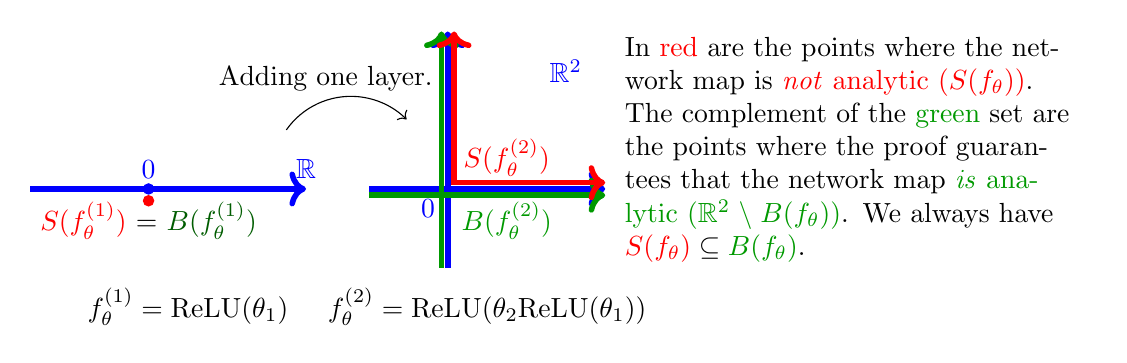
\begin{tikzpicture}[line width=2]
		\draw[color=blue, ->] (-1.5, 0) -- (2,0);
		\draw[color=blue, fill=blue, radius=1pt] (0, 0) circle;
		\node at (0, 0.25) {\textcolor{blue}{0}};
		\node at (2, 0.25) {\textcolor{blue}{$\mathbb R$}};

		\draw[color=red, fill=red, radius=1pt] (0, -0.15) circle;
		\node at (0, -0.4) {\textcolor{red}{$S(f^{(1)}_\theta)$} $ = $
		\textcolor{green!60!black!60!black}{$B(f^{(1)}_\theta)$}};

		\node at (0.5, -1.5) {\textcolor{black}{$f^{(1)}_\theta = \text{ReLU}(\theta_1)$}};

		\node at (2.25, 1.4) {Adding one layer.};
		\draw[black, thin, ->] (1.75, 0.75) arc (145:45:1);
	
		\begin{scope}[shift={(-0.2,0.0)}]
			\draw[color=blue, ->] (3, 0) -- (6,0);
			\draw[color=blue, ->] (4, -1) -- (4,2);
			\node at (3.75, -0.25) {\textcolor{blue}{0}};
			\node at (5.5, 1.5) {\textcolor{blue}{$\mathbb R^2$}};

			\draw[color=green!60!black, ->] (3, -0.08) -- (6, -0.08);
			\draw[color=green!60!black, ->] (3.92, -1) -- (3.92,2);
			\node at (4.75, -0.4) {\textcolor{green!60!black}{$B(f^{(2)}_\theta)$}};

			\draw[color=red, ->] (4.05, 0.08) -- (6, 0.08);
			\draw[color=red, ->] (4.08, 0.05) -- (4.08,2);
			\node at (4.75, 0.4) {\textcolor{red}{$S(f^{(2)}_\theta)$}};

			\node at (4.5, -1.5) {\textcolor{black}{$f^{(2)}_\theta = \text{ReLU}(\theta_2\text{ReLU}(\theta_1))$}};
		\end{scope}
		\node[text width=5.9cm] at (9.0, 0.5) {In \textcolor{red}{red} are the points where
				the network map is \textcolor{red}{\emph{not} analytic
				($S(f_\theta)$)}. \\The complement of the
				\textcolor{green!60!black}{green} set
			are the points where the proof guarantees that the network map
		\textcolor{green!60!black}{\emph{is} analytic ($\mathbb R^2 \setminus
	B(f_\theta)$)}. We always have $ \textcolor{red}{S(f_\theta)} \subseteq
\textcolor{green!60!black}{B(f_\theta)}. $};
	\end{tikzpicture}
	\caption{Illustration taken from paper}
\end{figure}
    

\end{frame}

\section{Extensions to Modern Architectures}

\begin{frame}{Beyond Fully Connected Networks}
    \begin{itemize}
        \item \textbf{Convolutional Neural Networks (CNNs):}
        \item Convolutions are strictly linear operations. The composition of linear operations with piecewise analytic activations follows the exact same stratification rules as dense layers.
        \item \textbf{Attention Layers (Transformers):}
        \item The Self-Attention mechanism relies on the Softmax function.
        \item Softmax is a composition of exponentials and (positive) division, which is strictly real analytic everywhere.
        \item Therefore, interleaving Softmax attention layers with ReLU-based MLPs (as in modern Transformers) maintains the piecewise analytic property of the total loss landscape.
    \end{itemize}
\end{frame}

\section{Conclusion}

% \begin{frame}{Bridging Theory and Practice}
%     \begin{itemize}
%         \item \textbf{Validation of Existing Theory:} Dozens of papers over the last decade assumed "non-singularity" or "Lipschitz smoothness" to prove optimization bounds. This paper retroactively validates those proofs for the actual networks practitioners use.
%         \item \textbf{Stochasticity:} Theorem 1 holds for any fixed mini-batch. Therefore, the Stochastic Gradient Descent (SGD) operator is a composition of non-singular maps (which remains non-singular).
%         \item \textbf{Momentum / Adam:} A natural extension is applying this framework to momentum-based optimizers. Because momentum updates are algebraic combinations of gradients, the same analytic stratification holds.
%     \end{itemize}
% \end{frame}

\begin{frame}{Conclusion}
    \begin{itemize}
        \item The GD map is mathematically well-behaved even when the loss landscape is fractured by ReLUs.
        \item Pathological behaviors (collapsing entire regions of parameter space into saddle points) are mathematically impossible for almost all learning rates.
        % \item Alexandru Crăciun and Debarghya Ghoshdastidar have provided a fundamental piece of foundational math for Deep Learning theory.
    \end{itemize}
\end{frame}

\begin{frame}
    \begin{center}
        \Huge \textbf{Thank You} \\
        \vspace{1cm}
        \Large \textit{Questions \& Discussion}
    \end{center}
\end{frame}

\end{document}
